\RequirePackage{luatex85}
\documentclass[tikz]{standalone}

\usepackage{tikz-feynman}

\begin{document}
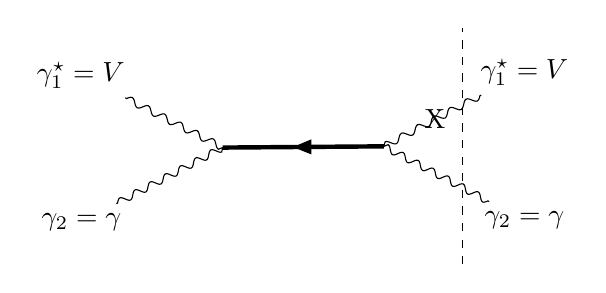
\begin{tikzpicture}
    \begin{feynman}
        \diagram [vertical=in1 to in2,medium] {
            x1 -- [fermion, ultra thick] x2,
            in1 [particle={\(\gamma_1^{\star} = V\)}] -- [photon] x1 [particle=a],
            in2 [particle={\(\gamma_2 = \gamma\)}] -- [photon] x1,
            out1 [particle={\(\gamma_1^{\star} = V\)}] -- [photon] x2,
            out2 [particle={\(\gamma_2 = \gamma\)}] -- [photon] x2,
            out1 -- [opacity=0] out2,
            in1 -- [opacity=0] in2,
        };
    \end{feynman}

    \begin{scope}[shift={(1, 0)}]
        \draw[dashed] (0, -1.5) -- (0, 1.5);
        \node at (-0.35, 0.35) {X};
    \end{scope}
\end{tikzpicture}
\end{document}
